\documentclass[./dokumentation.tex]{subfiles}

\begin{document}
\chapter{Potenzial von emotionalem Design}
Ob der Nutzer eine Beziehung zu einer Webseite oder einem Produkt aufbauen kann, hängt davon ab, ob die Erfahrung, die er mit dieser gemacht hat, angenehm oder nützlich war. Trevor van Gorp geht in \cite{vanGorp2013} sogar davon aus, dass der Grund für den Beziehungsaufbau zwischen Menschen vergleichbar ist. So soll man eher eine Beziehung aufbauen, wenn man den Besuch einer Webseite genießt und beim Verwenden dieser ein gutes Gefühl bekommt. Einen ähnlichen Effekt können auch attraktive Menschen haben. Ist eine Webseite dazu noch einfach zu bedienen und leicht zu verstehen, ist dies vergleichbar mit einem guten Gesprächspartner, zu dem man schneller eine Beziehung aufbaut. Wenn eine Webseite den Nutzer über einen längeren Zeitraum begleitet und zu seiner Zufriedenheit beiträgt, ist auch dies ein Faktor für das Aufbauen einer tiefen Beziehung, ähnlich wie auch Menschen sich an langfristige Beziehungen untereinander binden, um ihre (emotionalen) Bedürfnisse zu erfüllen (\cite{vanGorp2013}).

\section{Ebenen der emotionalen Verarbeitung}
Möchte man Nutzer emotional erreichen, ist es wichtig, die Ebenen der emotionalen Verarbeitung zu kennen und das User-Interface in diesen Bereichen entsprechend auszurichten. Dabei kann in drei verschiedene Ebenen unterschieden werden:
\begin{itemize}
    \item das viszerale emotionale Design
    \item das verhaltensbezogene emotionale Design
    \item das reflektive emotionale Design
\end{itemize}

Viszerales emotionales Design, also das limbische System betreffend, wird durch ein erstes sensorisches Erlebnis ausgelöst. Es ist der erste Eindruck eines Produkts und legt den Rahmen fest, in dem das weitere Erlebnis stattfindet. Viszerales Design hat, korrekt angewandt, einige positive Auswirkungen: Es setzt einen positiven Kontext für jede folgende Interaktion mit dem Produkt und baut eine positive Bindung zu einem Produkt auf. Durch dieses initial erreichte positive Erlebnis sind Nutzerinnen und Nutzer eher dazu bereit, Fehler an anderer Stelle des Produkts zu verzeihen.
Häufig werden bei digitalen Produkten gute Motion Designs verwendet, um ein vorsichtiges “onboarden” des Nutzers zum Produkt zu ermöglichen (\cite{medium_muz}).  

\begin{figure}[H]
    \centering
    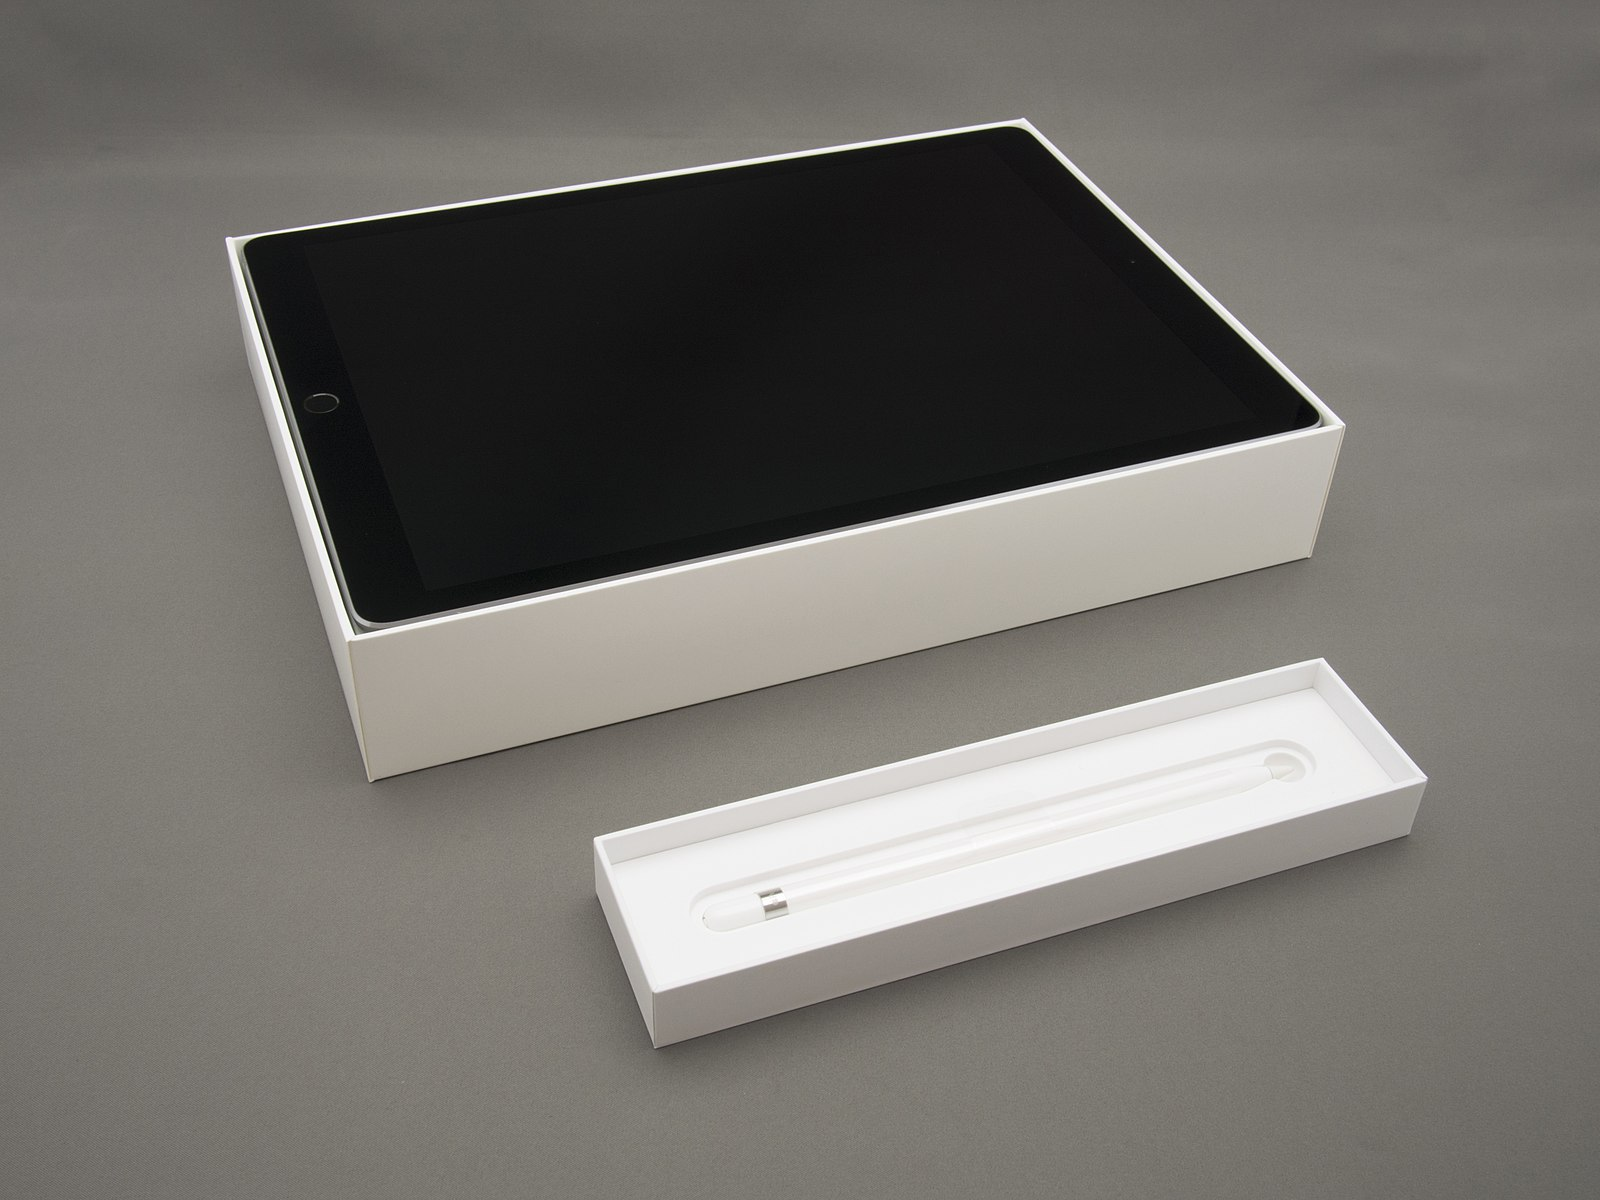
\includegraphics[width=0.8\textwidth]{bilder/ipadbox.jpg}
    \caption{Viszerale emotionale Reaktion (\cite*{ipadbox})}
    \label{fig1:visc}
\end{figure}


Verhaltensbezogenes emotionales Design erhöht die Eintauchtiefe, die ein Produkt einem Nutzer ermöglicht. Aus emotionaler Perspektive ermöglichen es flüssige, erwartungskonforme oder vertraute Interaktionen mit dem Produkt Zufriedenheit und Freude aus der Nutzung eines Produkts zu ziehen. Beim verhaltensbezogenen emotionalen Design kommt es sowohl auf Funktion, als auch auf Performance und Effektivität an.
Starke positive Reaktionen haben an dieser Stelle ebenso mehrere Auswirkungen: Wir fühlen uns des Produkts mächtig und kompetent und bauen ein Vertrauensverhältnis zum Produkt auf, indem eine direkte Korrelation zwischen den Aktionen und Reaktionen geschaffen wird. Darüber hinaus motivieren diese Erfolgserlebnisse, das Produkt erneut zu nutzen, um erneut eine positive Erfahrung zu erleben (\cite{medium_muz}).\pagebreak


\begin{figure}[H]
    \centering
    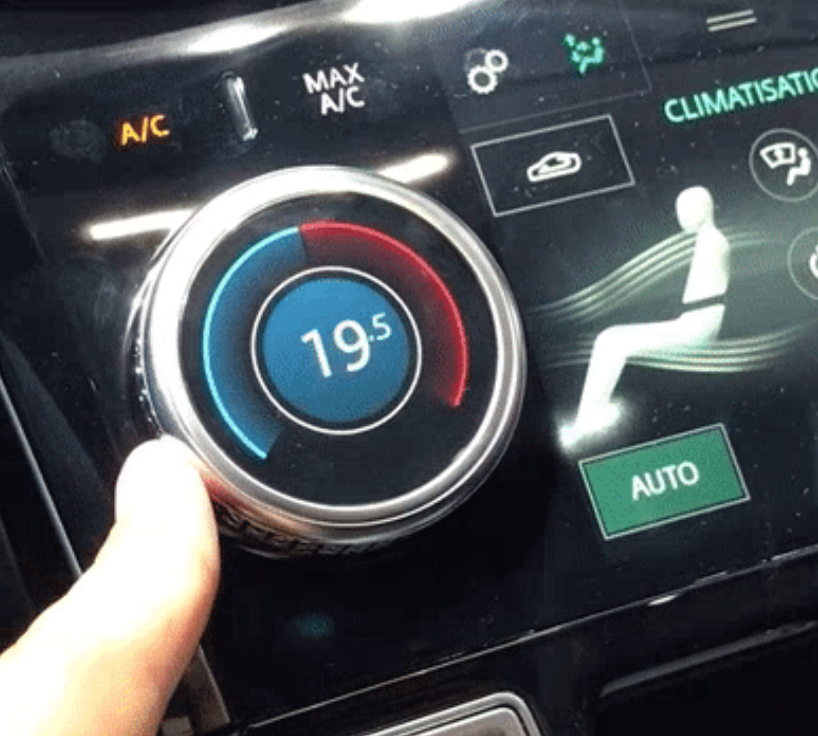
\includegraphics[width=0.5\textwidth]{bilder/verh-bez-des.png}
    \caption{Verhaltensbezogenes emotionales Design (\cite{medium_muz})}
    \label{fig2:verh}
\end{figure}\\

Reflektives emotionales Design beschreibt, wie wir uns nach der Nutzung eines Produkts, unmittelbar nach einer durchgeführten Interaktion fühlen. Hierdurch wird bestimmt, wie die Erinnerungen an das Produkt sein werden. Wollen wir etwas erneut nutzen, oder interessiert es uns in Zukunft weniger? Positive, reflektive Reaktionen motivieren uns, Erfahrungen mit anderen zu teilen. Sie rufen eine Identifikation mit dem Produkt hervor (\cite{medium_muz}).\\

\begin{figure}
    \centering
    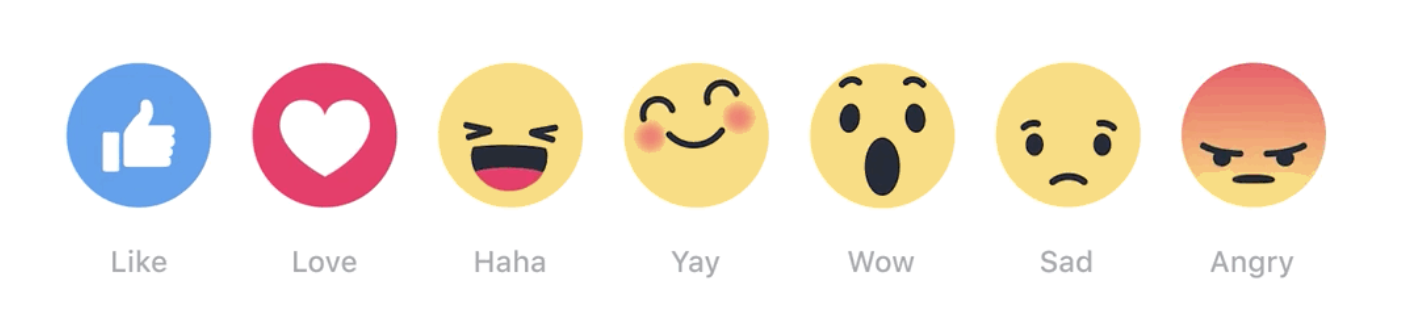
\includegraphics[width=0.8\textwidth]{bilder/refl-design.png}
    \caption{Reflektives emotionales Design (\cite{medium_muz})}
    \label{fig3:refl}
\end{figure}\pagebreak

Um die Emotionen der Nutzerschaft zu erreichen, können unter anderem die folgenden Elemente eingesetzt werden: 
\begin{itemize}
    \item Personalisierung und Anpassung
    \subitem{} durch die Personalisierung wird erreicht, dass Nutzer sich verantwortlich und eingebunden fühlen
    \item Humor
    \subitem{} Lachen und Freude sind sehr starke emotionen, die Unsicherheiten lindern und einen positiven bleibenden Eindruck hinterlassen
    \item Storytelling
    \subitem{} Storytelling hilft dabei, das Nutzererlebnis selbst zu verstehen und eine Erinnerung an das Produkt zu schaffen
    \item positive Überraschungen
    \subitem{} positive Emotionale Reaktionen können hervorgerufen werden, in dem Nutzer freudvoll überrascht werden
\end{itemize}

%\subsection{Emotionen - Grundlagen}
\end{document}


